\documentclass[11pt]{article}
\usepackage{graphicx}
\DeclareGraphicsExtensions{.png,.jpg}
\graphicspath{{./figures/}}
\usepackage{url}

\begin{document}

\title{Architecture of the Proposed Cloud Application Platform Monitor}
\author{Hiranya Jayathilaka, Wei-Tsung Lin, Chandra Krintz, and 
Rich Wolski \\
Computer Science Dept., UC Santa Barbara \\
\\
Collaborators: Michael Xie and Ying Xiong \\
Huawei Technologies\\
\\
January 2016
}
\date{}
\maketitle

\section{Introduction}
Over the last decade Platform-as-a-Service (PaaS) has become a popular approach for deploying
applications in the cloud. Many organizations, academic institutions, and hobbyists make use of public
and/or private PaaS clouds to deploy their applications.
PaaS clouds provide a high level of abstraction to the application developer that effectively hides
all the infra\-structure-level details such as physical resource allocation (CPU, memory, disk etc), operating
system,
and network configuration. This enables application developers to focus solely on the programming
aspects of their applications, without having to be concerned about deployment issues. 

PaaS clouds execute web-accessible (HTTP/s) applications, to which they provide high levels of scalability, availability, and execution management. 
PaaS clouds provide scalability by automatically allocating resources 
for applications on the fly (auto scaling), and provide availability through
the execution of multiple instances of the application and/or the PaaS
services they employ for their functionality.
Consequently, viable PaaS technologies as well as
PaaS-enabled applications continue to increase rapidly in number.

This rapid growth in PaaS technology has intensified the need 
for new techniques to
monitor applications deployed in a PaaS cloud. Application developers and users wish
to monitor the availability of the deployed applications, track application performance, and detect 
application and system anomalies as they occur. To obtain this level of deep operational insight into
PaaS-deployed applications, the PaaS clouds must be equipped with powerful instrumentation,
data gathering and analysis capabilities that span the entire stack of the PaaS cloud. 
Moreover, PaaS clouds must provide comprehensive
data visualization and notification mechanisms. However, most PaaS technologies available
today either do not provide any application monitoring support, or only provide primitive
monitoring features such as application-level logging. Hence, they are not capable of performing
powerful predictive analyses or anomaly detection, which require much more fine-grained, low-level
and full stack data collection and analytics. 

To address this limitation, we present the design of 
a comprehensive application platform 
monitor (APM) that can be easily integrated with a wide variety of PaaS technologies. The proposed
APM is not an external system that monitors a PaaS cloud from the outside (as most APM systems today). Rather, it integrates with
the PaaS cloud from within thereby extending and augmenting the existing components of the PaaS cloud
to provide comprehensive full stack monitoring, analytics and visualization capabilities. We believe that this design decision is a key differentiator over existing PaaS and cloud application monitoring systems because (i) it is
able to take advantage of the scaling, efficiency, deployment, fault tolerance, security, and control features that the PaaS offers, (ii) while providing low overhead end-to-end monitoring and analysis of cloud applications.

This document details the architecture of the proposed APM, and how it integrates with a typical PaaS
cloud. We describe individual components of the APM, their functions and how they interact with each
other. Where appropriate, we also detail the concrete technologies (tools and products) that we plan to use to implement
various components of the APM, and provide our rationale and intuition behind choosing these technologies.

We start by describing the layered system organization typically seen in PaaS clouds. Then we describe
the APM architecture, and show how it fits into the PaaS.

\section{PaaS System Organization}
\begin{figure}
\centering
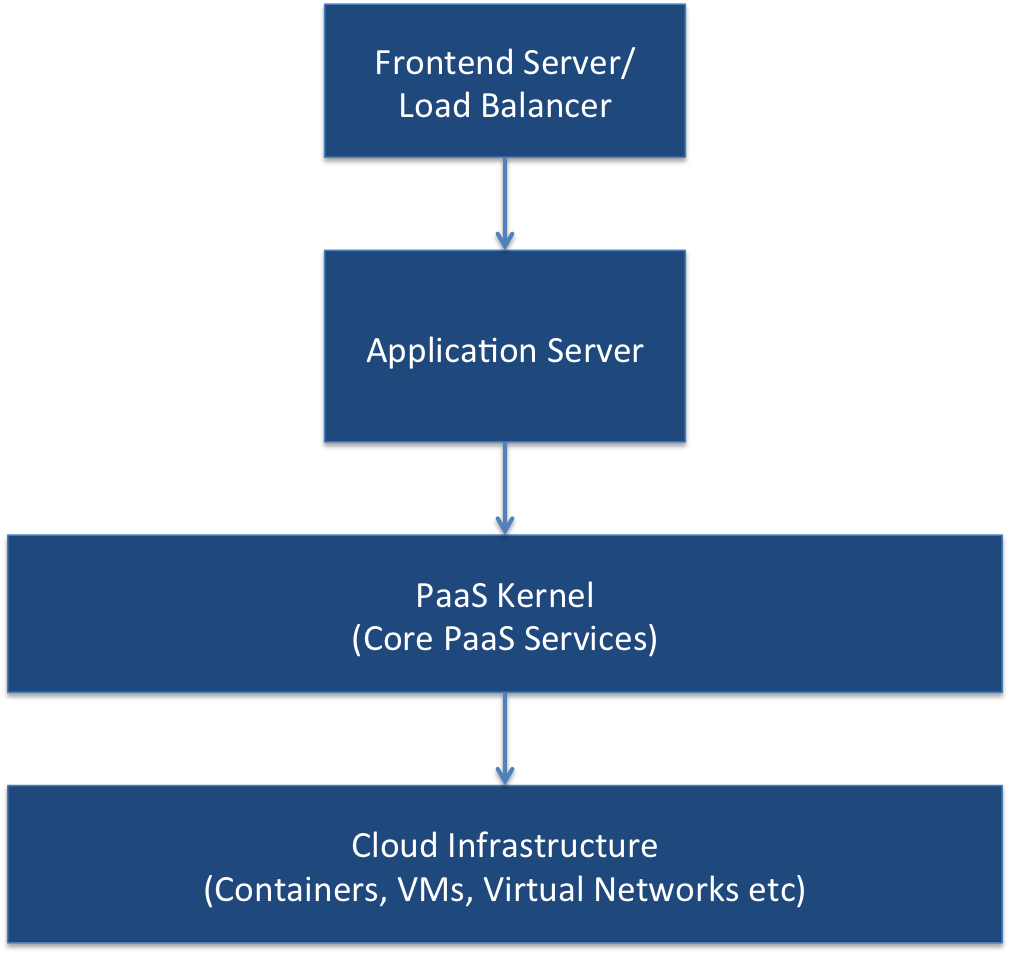
\includegraphics[scale=0.5]{paas_architecture}
\caption{PaaS system organization.}
\label{fig:paas_architecture}
\end{figure}

Figure~\ref{fig:paas_architecture} shows the key system layers of a typical PaaS cloud. Arrows indicate
the flow of data and control in response to application requests.

At the lowest level of a PaaS cloud is an infrastructure that consists of the necessary compute, storage
and networking resources. How this infrastructure is set up may vary from a simple cluster of physical 
machines to a comprehensive Infrastructure-as-a-Service (IaaS) solution. In large scale PaaS clouds,
this layer typically consists of many virtual machines and/or containers with the ability to acquire more
resources on the fly.

On top of the infrastructure layer lies the PaaS kernel. This is a collection of managed, scalable
services that high-level application developers can compose into their applications. The provided services
may include database services, caching services, queuing services and much more. Some PaaS clouds
provide a managed set of APIs (an SDK) for the application developer to access these fundamental services. 
In that case all interactions between the applications and the PaaS kernel must take place through
the cloud provider specified APIs (e.g. Google App Engine). 

One level above the PaaS kernel we find the application servers that are used to deploy and run
applications. Application servers provide the necessary integration (linkage) between application code and the
underlying PaaS kernel, while sandboxing application code for secure, multi-tenant operation. On top
of the application servers layer resides the fronted and load balancing layer. This layer is responsible
for receiving all application requests, filtering them and routing them to an appropriate application
server instance for further execution. As the fronted server, it is the entry point for PaaS-deployed
applications for all application clients.

\section{Cloud APM Architecture}
\subsection{Key Functions}
\begin{figure}
\centering
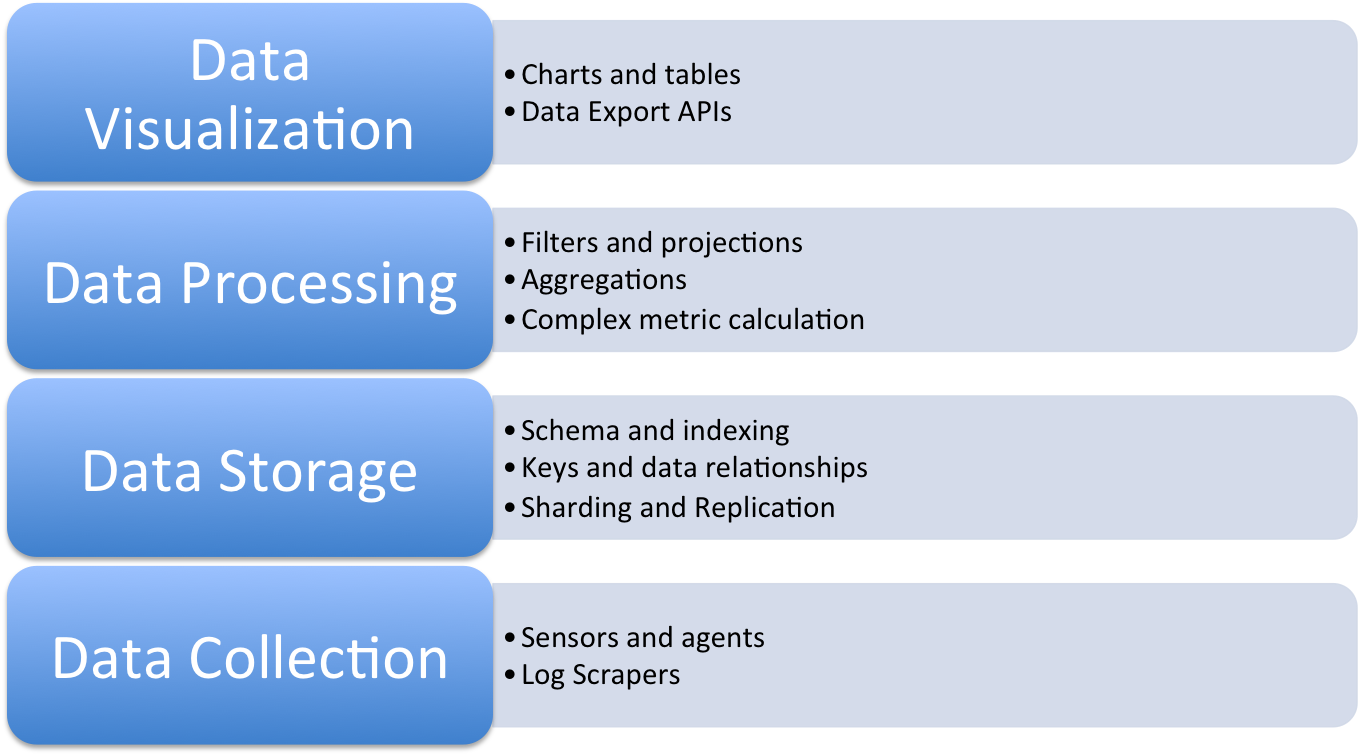
\includegraphics[scale=0.5]{apm_functions}
\caption{Key functions of the APM.}
\label{fig:apm_functions}
\end{figure}

\begin{figure}
\centering
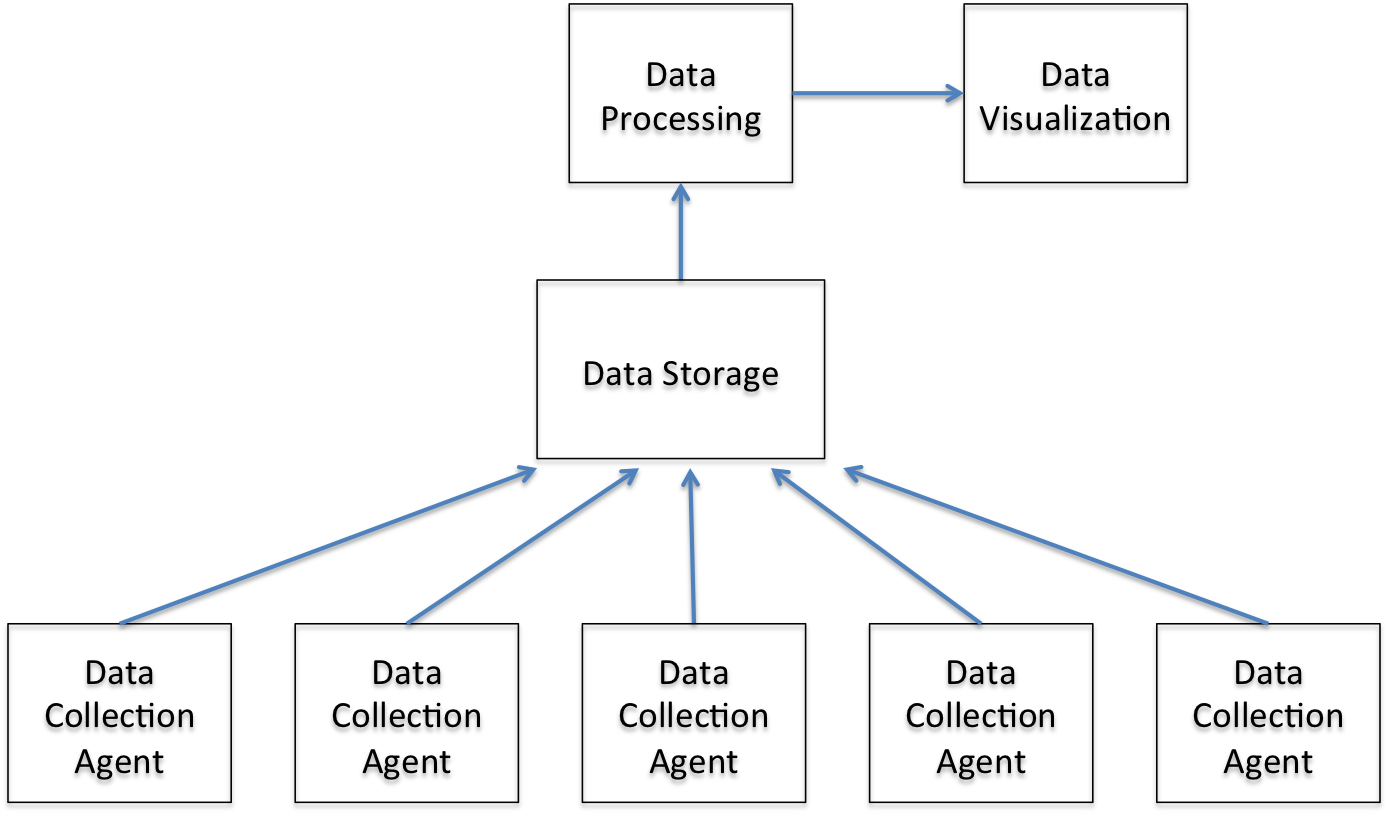
\includegraphics[scale=0.5]{apm_layout}
\caption{Deployment view of the APM functions.}
\label{fig:apm_layout}
\end{figure}

Like most system monitoring solutions, the proposed cloud APM must serve four major functions: Data
collection, storage, processing (analytics) and visualization. Figure~\ref{fig:apm_functions} shows the
logical organization of these functions in the APM, and various tasks that fall under each of them.
Figure~\ref{fig:apm_layout} shows a physical deployment view of the said functions. Arrows indicate
the flow of information through the APM.

Data collection is performed by various sensors and agents that instrument the applications and the
core components of the PaaS cloud. While sensors are very primitive in their capability to monitor
a given component, an agent may intelligently adapt to changing conditions, making decisions on
what information to capture and how often. Monitoring and instrumentation should be lightweight and as non-intrusive
as possible so their existence does not impose additional overhead 
on the applications.

Data storage components should be capable of
dealing with potentially very high volumes of data. The data must be organized and indexed
to facilitate efficient retrieval, and replicated to maintain reliability and high availability. 

Data processing components should also be capable of processing large volumes of data in near real-time,
while supporting a wide range of data analytics features such as filters, projections and aggregations. 
They will employ various statistical and perhaps even machine learning methods to understand the
data, detect anomalies and identify bottlenecks in the system.

Data visualization layer mainly consists of graphical interfaces (dashboards) for displaying various
metrics computed by the data processing components. Additionally it may also have APIs to export
the calculated results and trigger alerts. 

\subsection{APM Architecture and Integration with PaaS}
\begin{figure}
\centering
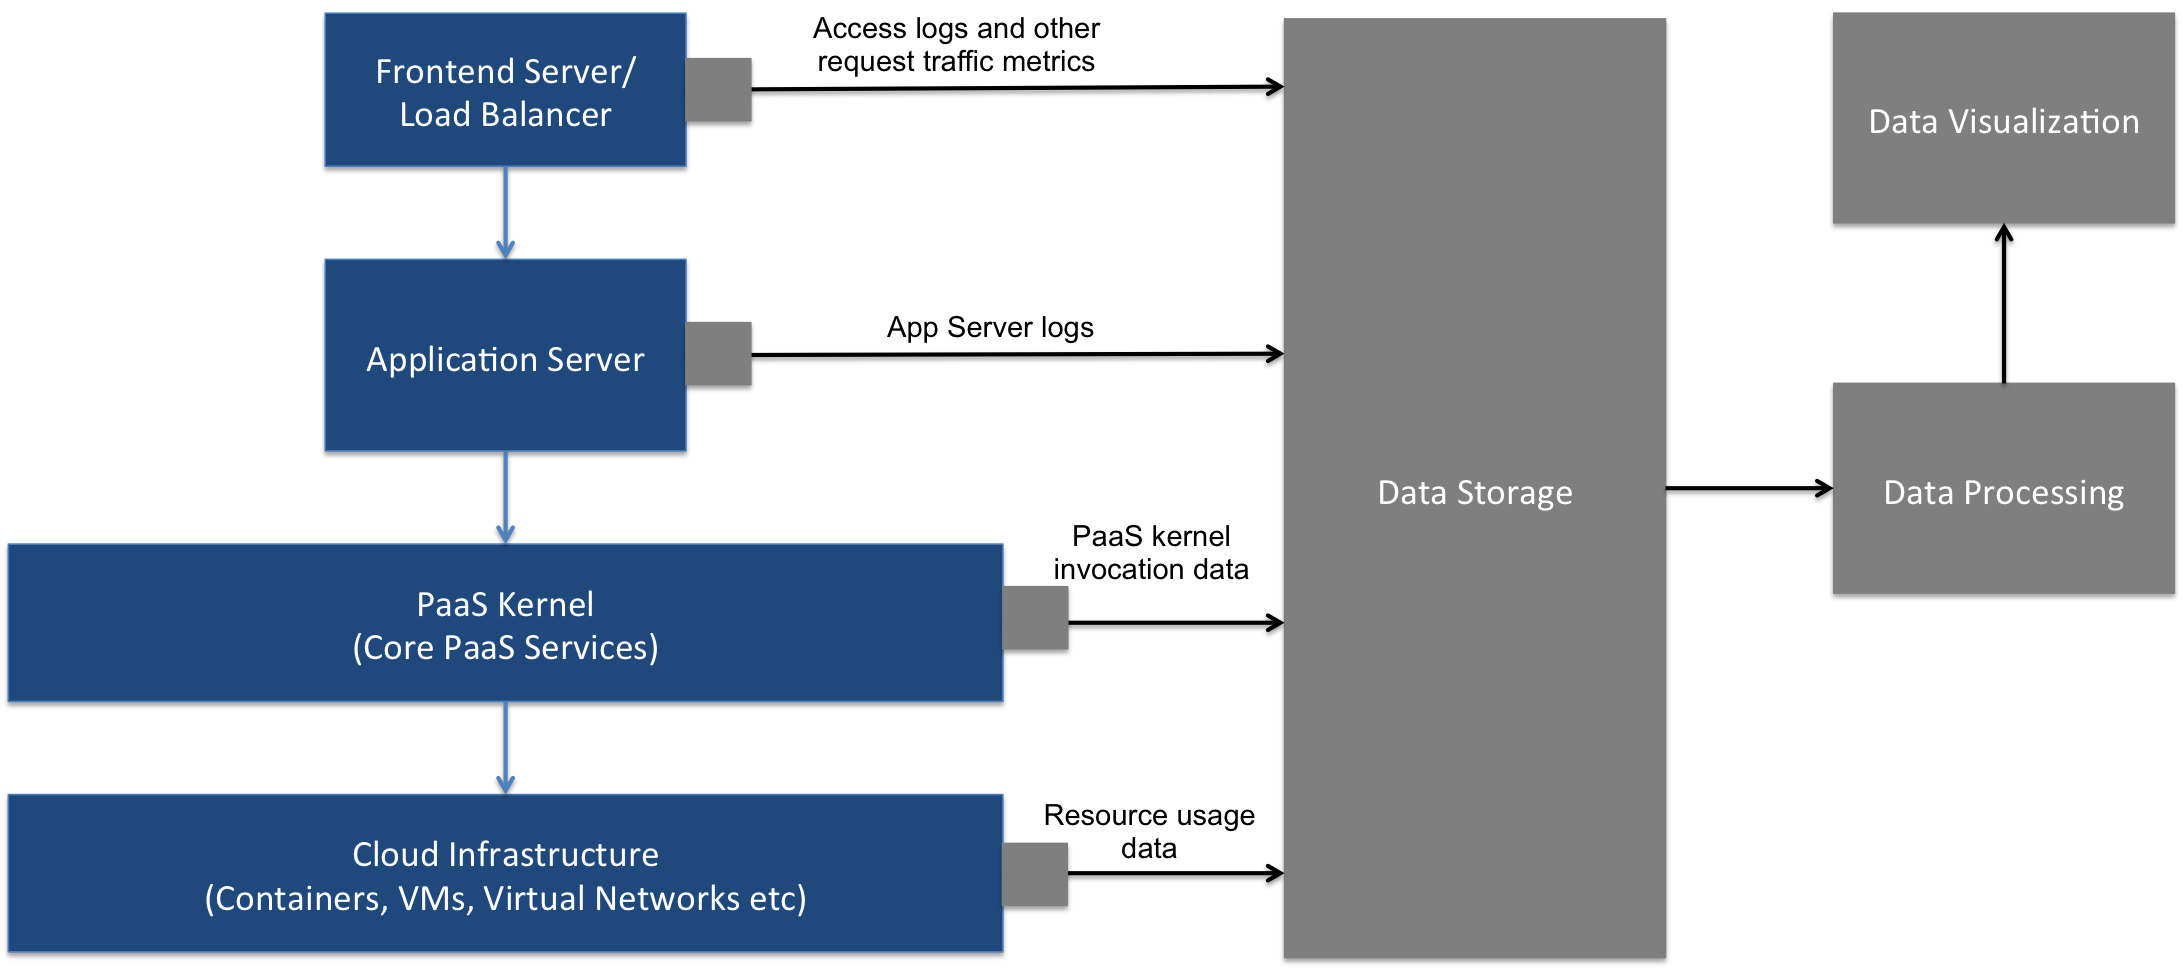
\includegraphics[scale=0.35]{apm_architecture}
\caption{APM architecture.}
\label{fig:apm_architecture}
\end{figure}

Figure~\ref{fig:apm_architecture} illustrates the overall architecture of the proposed APM, and how 
it fits into the PaaS cloud stack. APM components are shown in grey, with their interactions indicated
by the black lines. The small grey boxes attached to the PaaS components represent the sensors and
agents used to instrument the cloud platform for data collection purposes. Note that the APM collects
data from all layers in the PaaS stack (i.e. full stack monitoring).

From the front-end and load balancing layer we gather all information related to incoming application
requests. A big part of this is scraping the HTTP server access logs, which indicate request timestamps,
source and destination addressing information, response time (latency) and other HTTP message
parameters. This information is readily available for harvesting in most technologies used as front-end
servers (e.g. Apache HTTPD, Nginx). Additionally we may also collect information pertaining to active
connections, invalid access attempts and other errors.

From the application server layer we intend to collect basic application logs as well as any other logs and 
metrics that can be easily collected from the application runtime. This may include some process level
metrics indicating the resource usage of the individual application instances. If deeper insight into the 
application execution becomes necessary, more intrusive instrumentation can be introduced to the 
application server (perhaps selectively or adaptively). 

At the PaaS kernel layer we employ instrumentation to record information regarding all kernel invocations
made by the applications. This instrumentation must be applied carefully as to not introduce a noticeable
overhead to the application execution. For each PaaS kernel invocation, we can capture the 
following parameters.
\begin{itemize}
\item Source application making the kernel invocation
\item Timestamp
\item Target kernel service and operation
\item Execution time of the invocation
\item Request size, hash and other parameters
\end{itemize}
Collecting this PaaS kernel invocation details enables tracing the execution of application 
requests, without the need for instrumenting application code, which we believe is a feature 
unique to PaaS clouds. 

Finally, at the lowest infrastructure level, we can collect information related to virtual machines, containers
and their resource usage. We can also gather metrics on network usage by individual components which
might be useful in a number of traffic engineering use cases. Where appropriate we can also scrape
hypervisor and container manager logs to get an idea of how resources are allocated and released over
time.

To summarize, the types of services and resources that this APM will be able
to monitor include the following. Moreover, our design of the data collection layer is abstract and thus easily extended to permit monitoring of new services and PaaS components as they become available in the future.
\begin{itemize}
\item Cloud Infrastructure: 
\begin{itemize}
\item CPU, memory, disk, network
\item Linux containers, virtual machines
\end{itemize}
\item PaaS Kernel (including PaaS cloud SDK)
\begin{itemize}
\item Task queues, security components (user/developer tracking and authentication and authorization), enterprise service bus
\item Data caches (memcache), datastores (key value, NoSQL), databases (fixed schema, SQL).
\end{itemize}
\item Application servers
\begin{itemize}
\item Per-language runtime systems
\item Our APM will target the Java language
\end{itemize}
\item Front-end components
\begin{itemize}
\item HTTP/s request serving 
\item Load balancing and rate limiting components
\end{itemize}
\end{itemize}

\subsection{Cross-layer Data Correlation}
Previous subsection details how the APM collects useful monitoring data at each layer of the cloud
stack. To make most out of the gathered data, and use them to perform complex analyses, we must be able to correlate data records collected at different layers of the PaaS. For example consider
the execution of a single application request. This single event results in following data records at
different layers of the cloud, which will be collected and stored by the APM as separate entities.

\begin{itemize}
\item A front-end server access log entry
\item An application server log entry
\item Zero or more application log entries
\item Zero or more PaaS kernel invocation records
\end{itemize}

We require a mechanism to tie these disparate records together, so the data processing layer can easily
aggregate the related information. For instance, we must be able to retrieve via an
aggregation query, all PaaS kernel invocations made by a specific application request.

To facilitate this requirement we propose that front-end server tags all incoming application requests 
with unique identifiers.
This request identifier can be attached to HTTP requests as a header which is visible to all components 
internal to the PaaS cloud. All data collecting agents can then be configured to record the request identifiers
whenever recording an event. At the data processing layer APM can aggregate the data by request identifiers
to efficiently group the related records.

\section{Implementation}
\begin{figure}
\centering
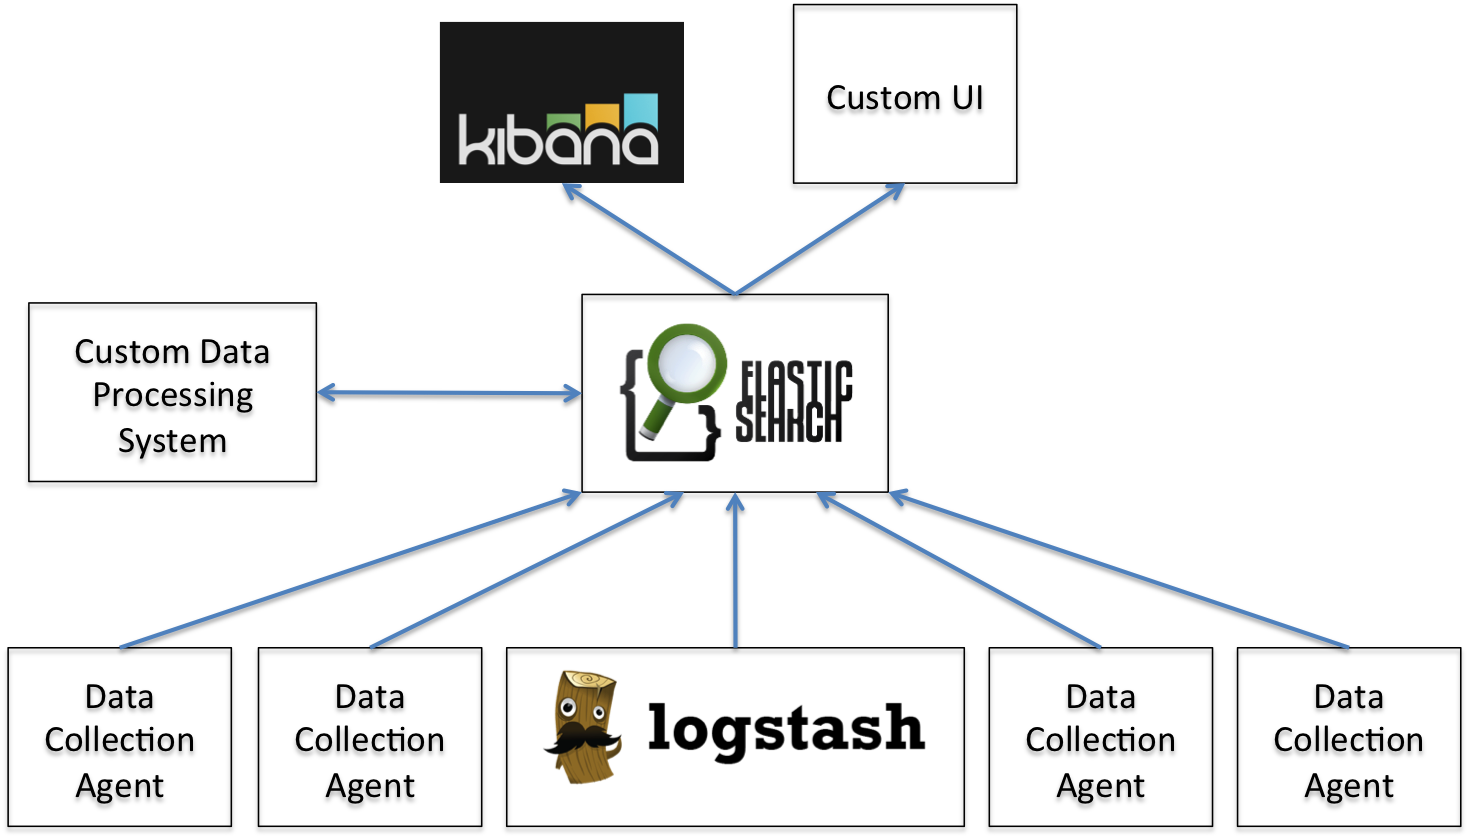
\includegraphics[scale=0.5]{apm_impl}
\caption{APM implementation based on ElasticSearch.}
\label{fig:apm_impl}
\end{figure}
In this section we outline some of the technologies and tools that we have chosen to implement the proposed
APM architecture.  After a thorough evaluation of numerous existing system monitoring tools and platforms, 
we have decided to implement our APM for PaaS clouds using ElasticSearch. More specifically, ElasticSearch
will operate as the primary data storage component of the APM. ElasticSearch is ideal for storing large volumes
of structured and semi-structured data. It supports scalability and high availability via sharding and replication.
Perhaps what makes ElasticSearch an excellent choice for an APM is its comprehensive data indexing and
query support. Using the tried and tested Apache Lucene technology, ElasticSearch continuously organizes
and indexes data, making the information available for fast retrieval and efficient querying. 
Additionally it also provides
powerful data filtering and aggregation features, which can greatly simplify the implementations of high-level
data processing algorithms.

Data can be directly stored in ElasticSearch via its REST API. This means most data collection agents can 
simply make HTTP calls to ElasticSearch to add new records. ElasticSearch also supports batch 
processing thereby enabling agents to locally buffer collected data, and store them in batches to avoid
making too many HTTP calls. For scraping server logs and storing the extracted records in ElasticSearch,
we can use the Logstash tool. Logstash supports scraping a wide range of standard log formats (e.g. 
Apache HTTPD access logs), and other custom log formats can be supported via a simple configuration.
It also integrates naturally with ElasticSearch.

For data visualization we are currently considering Kibana, a powerful web-based dash boarding tool 
that is specifically designed to operate in conjunction with ElasticSearch. Kibana provides a wide
range of charting and tabulation capabilities, with particularly strong support for temporal data.  Since
ElasticSearch exposes all stored data via its REST API, it's also possible to bring other visualization
tools into the mix easily.

Figure~\ref{fig:apm_impl} shows the APM deployment view with ElasticSearch and other related technologies
in place. Most of the data processing features are provided by ElasticSearch itself, and other more complex
data analytics can be provided by a custom data processing system. 

\section{APM Use Cases}
In this section we elaborate on some concrete use cases of the proposed APM. In particular, we discuss how
the APM can be used to predict performance SLAs for web applications deployed in a PaaS cloud, as well
as to detect performance anomalies. These use cases rely on the data collected by the APM, and some
of its data processing and visualization capabilities. Where appropriate we will extend the base design
of the APM to incorporate new components and tools required to implement the features discussed here.

\subsection{Static Topology Discovery and SLA Prediction}
Our goal is to give a prediction that can make it possible to determine response time service level agreements (SLAs)
with probabilities specified by the cloud provider in a way that is scalable.

To allow PaaS administrators to determine what response time guarantees can be made
regarding the deployed applications,
we will take an approach that combines static analysis of the hosted web applications and runtime monitoring of the PaaS cloud. 
Also, since we want to provide the prediction to PaaS users when they are deploying the applications,
such static analysis must be done before deploying or running an application on the PaaS cloud. 

A typical PaaS cloud exports many kinds of services, such as data storage, caching and queuing (PaaS kernel
services). Application developers
compose these services into their web applications. 
From experience, we know that most applications hosted on PaaS spend majority of
the execution time on PaaS service invocations, and they do not have many branches and loops. Therefore, in our design we use
static analysis to identify the PaaS kernel service invocations that dominate the response time of web applications.
By doing so we also detect the topology of applications -- i.e. the service dependencies.

Our APM design includes sensors/agents that monitor the performance of PaaS kernel services over time. This
information can be recorded periodically to form a set of time series. This historical performance data can be
aggregated and processed using a time series forecasting methodology to calculate statistical bounds on the
response time of applications. These forecast values can be used as the basis of
a performance SLA.
Also, because service implementations and platform behavior under load change over time,
the predicted SLAs may become invalid after a period of time. We will develop a statistical model to detect such SLA invalidations.
When such invalidations occur, the SLA prediction can be reinvoked to establish new SLAs.

To build a system that predicts response time SLAs using only static information, our design has three components:
\begin{itemize}
\item Static analysis tool
\item Monitoring agent
\item SLA predictor
\end{itemize}

\subsubsection{Static Analysis Tool}
\begin{figure}
\centering
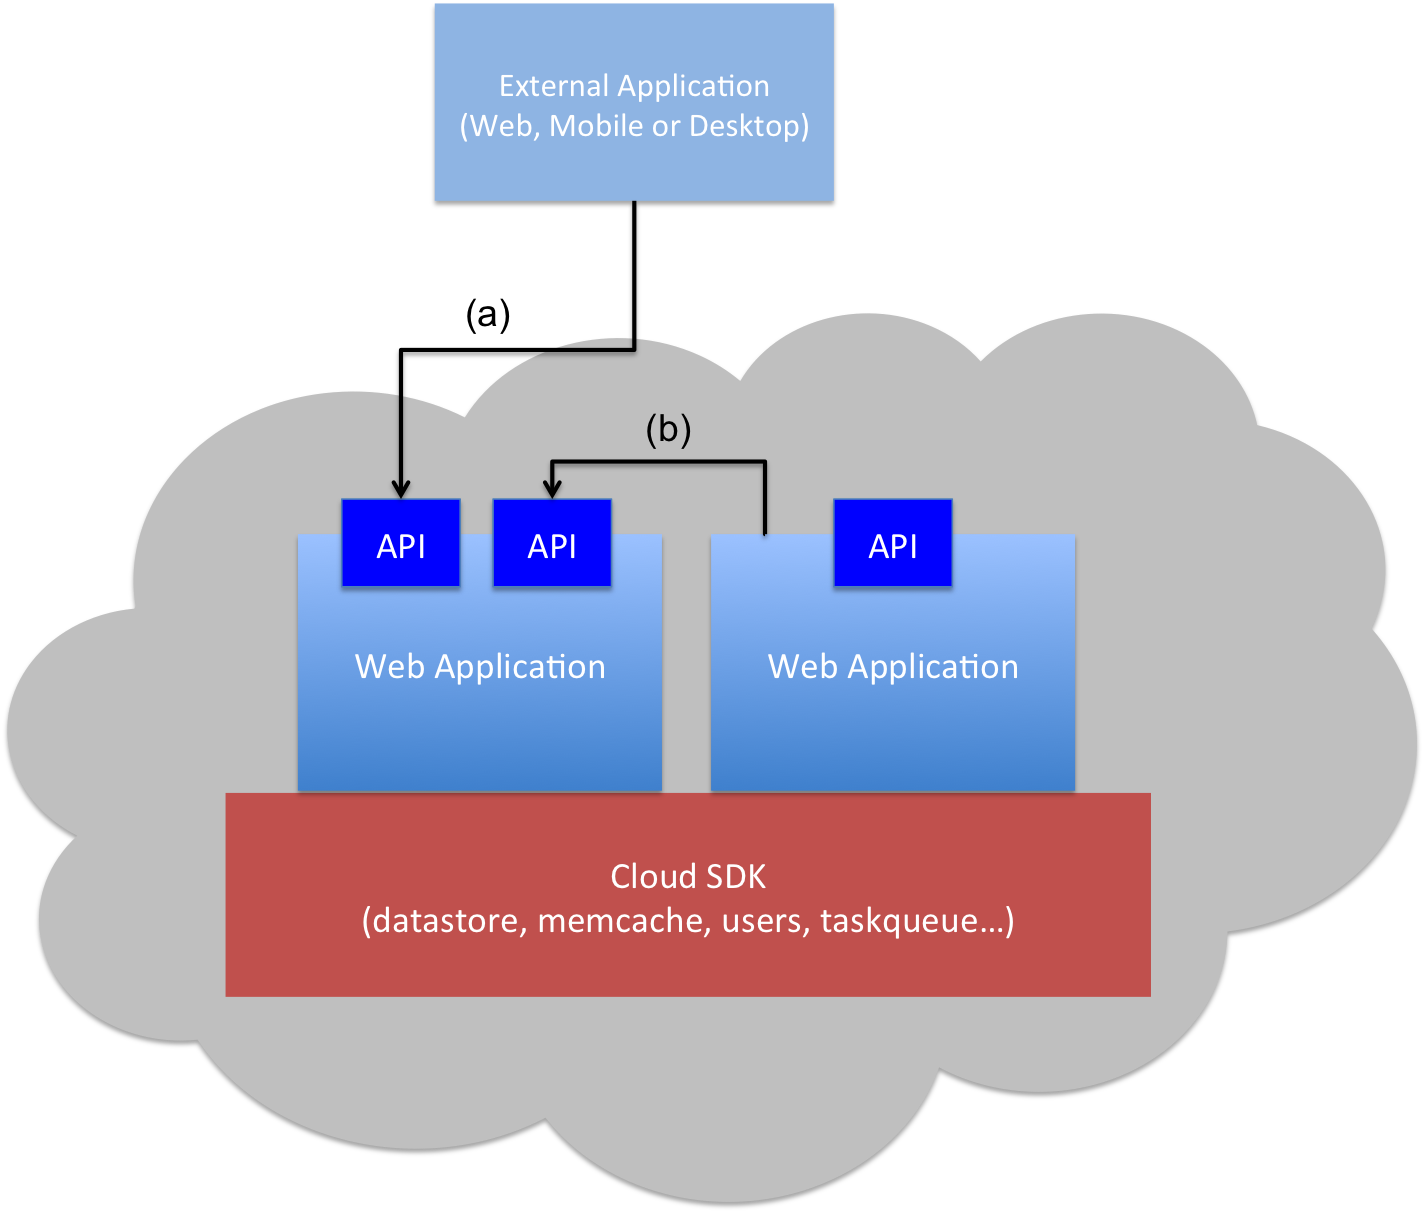
\includegraphics[scale=0.4]{cloud_app_model}
\caption{Cloud Application Model.}
\label{fig:cloud_app_model}
\end{figure}

This component analyzes the source code of the web application and extracts a sequence of PaaS service invocations.

Figure~\ref{fig:cloud_app_model} illustrates the typical PaaS development and deployment model. 
Developers use the services exposed by the
PaaS cloud (aka PaaS kernel services or PaaS SDK) to implement their applications. Applications
in turns are exposed to end users via one or more web APIs. The end user could be a client application
external to the cloud, or another application running in the same cloud environment. 
The underlying PaaS kernel service implementations are highly scalable, highly available
(have SLAs associated with them), and automatically managed by the platform. 
Developers upload their finished applications to the cloud for deployment. An uploaded
application typically consists of source code or some intermediate representation of it along
with one or more deployment descriptors (configurations, versioning information, crypto resources etc.)

When an application has been uploaded, the static analysis tool can analyze the source code 
or the application's intermediate representation (e.g. Java bytecode). It performs a simple 
construction and inter-procedural static analysis of the control flow graph (CFG).
By performing a depth-first traversal on the CFG it is possible to identify all possible paths
of execution through the application code. This includes paths that occur due to branching (if-else constructs, 
switch statements etc.), looping as well error handling (try-catch constructs). 
For each identified path, the static analysis tool extracts a sequence of PaaS service 
invocations. Since the applications need to be exposed to users through HTTP/s, 
the static analysis tool can begin the extraction by checking specific language classes
or framework annotations, for example, Java's servlet classes or the classes marked with
the JAX-RS Path annotation.

For each application the static analysis tool produces a list of annotated PaaS 
service invocation sequences -- one sequence per program path.
It then prunes this list to eliminate duplicates. Duplicates occur when an application has multiple program
paths with the same sequence of PaaS service invocations.
Ideally, we can identify the PaaS kernel service calls by their namespace 
(in Java's case, the package name).

Although loops are rare in this type of applications, when they occur, they are used to 
iterate over a dataset returned from a database. The tool estimates the loop 
bounds if specified in the PaaS kernel service API (e.g. the maximum number of entities to return). 
Otherwise, we can ask users to provide an estimation of the size of their dataset.

\subsubsection{Monitoring Agent}
This agent monitors and records the response time of individual PaaS services within a running PaaS system.

It can be built as a native PaaS feature, or as an independent application deployed on PaaS. To avoid unnecessary
performance overhead on other PaaS-hosted web applications, the monitoring agent runs in the background separate from them.
The agent invokes services provided by PaaS kernel periodically and records response times for each service. Also, the agent periodically
reclaims old measurement data to eliminate unnecessary storage.

In our design, these agents can be implemented as ElasticSearch's custom agents. The collected data will be sent back to ElasticSearch
and wait for processing.

\subsubsection{SLA predictor}
The SLA predictor uses the outputs of other two components to predict an upper bound 
on the response time of the services.
To make SLA predictions, we propose using Queue Bounds Estimation from Time Series 
(QBETS)~\cite{Nurmi:2007:QQB:1791551.1791556}, 
a non-parametric time series analysis method that we developed in prior work. 
We originally designed QBETS for
predicting the scheduling delays of batch queue systems 
used in high performance computing environments. 
We adapt it for use ``as-a-service'' in PaaS systems 
to predict the execution time of deployed applications.

A QBETS analysis requires three inputs:
\begin{enumerate}
\item A time series of data generated by a continuous experiment,
\item The percentile for which an upper bound should be predicted ($p \in [1..99]$)
\item The upper confidence level of the prediction ($c \in (0,1)$)
\end{enumerate}

QBETS uses this information to predict an upper bound for 
the $p$-th percentile of the input time series.
The predicted value has a probability of $0.01p$ of 
being greater than or equal to the next data point that
will be added to the time series by the continuous experiment. 
The upper confidence level $c$ serves as a conservative
bound on the predictions. That is, predictions made with an upper confidence 
level of $c$ will overestimate
the true percentile with a probability of $1-c$. This confidence guarantee 
is necessary because 
QBETS does not determine the 
percentiles of the time series precisely, but only estimates them.

To further clarify what QBETS does, assume a continuous experiment 
that periodically measures the
response time of a system. This results in a time series of 
response time data. Suppose at time $t$,
we run QBETS on the time series data collected so far 
with $p=95$ and $c=0.01$. The prediction returned
by QBETS has a 95\% chance of being greater than or equal 
to the next response time value measured
by our experiment after time $t$. Since $c=0.01$, the predicted value has a 99\% chance of
overestimating the true 95th percentile of the time series.

We find QBETS to be an ideal fit for our work due to several reasons. 
\begin{itemize}
\item QBETS works with time series data. Since the response time
of various PaaS kernel services can be easily represented as time series,
they are highly amenable for QBETS analysis. 
\item QBETS makes predictions regarding the
future outcomes of an experiment by looking at the past 
outcomes -- an idea that aligns with our
goal of predicting future application response times from historical PaaS kernel service performance data. 
\item Response time
SLAs of web applications should be specified with exact correctness 
probabilities and confidence levels for
them to be useful to developers and PaaS administrators. QBETS meets these requirements.
\item QBETS is 
simple, efficient and has been applied successfully to analyze a wide range of time series 
data, including correlated and uncorrelated data, in the past.
\end{itemize}

In our case, QBETS takes the response times for each PaaS kernel service 
we record in ElasticSearch.
Notice that this data is collected continuously by the PaaS monitoring agent, 
so QBETS is able to automatically adapt to the changing conditions of the cloud. 
Given the percentile for which 
an upper bound should be predicted and the upper confidence level of the prediction, 
QBETS can generate a conservative prediction. 

Since an application may invoke multiple PaaS kernel services, the SLA predictor also needs
to align and aggregate multiple time series together before engaging QBETS. For example, suppose
an application makes 3 PaaS kernel service invocations. The static analysis component would detect the
3 target kernel services invoked by the application. The SLA predictor should then retrieve the response time
data pertaining to those 3 PaaS kernel services from ElasticSearch. This information would be retrieved as
3 separate time series. SLA predictor then aligns the time series data (by timestamp), and aggregates them
to form a single time series where each data point is an approximation of the total time spent by the application
on invoking PaaS kernel services. This aggregate time series can be provided as the input to QBETS to
make the response time predictions.

Note that our static analysis tool produces multiple sequences of PaaS service invocations for each
analyzed application. Multiple sequences occur due to the existence of branches, loops and error handling
logic in the application code. The SLA predictor can make predictions for each of the paths identified
by the static analysis tool.  The largest predicted value can then be used as the basis for a response time
SLA, thus covering all paths of the input applications.

The key assumption that makes our approach viable is that PaaS-hosted web applications spend most of
their execution time on invoking PaaS kernel services. 
Previous studies~\cite{Jayathilaka:2015:RTS:2806777.2806842} have shown this to be true,
with applications spending over 90\% of their execution time on PaaS kernel service invocations.

\subsubsection{Workflow}
\begin{figure}
\centering
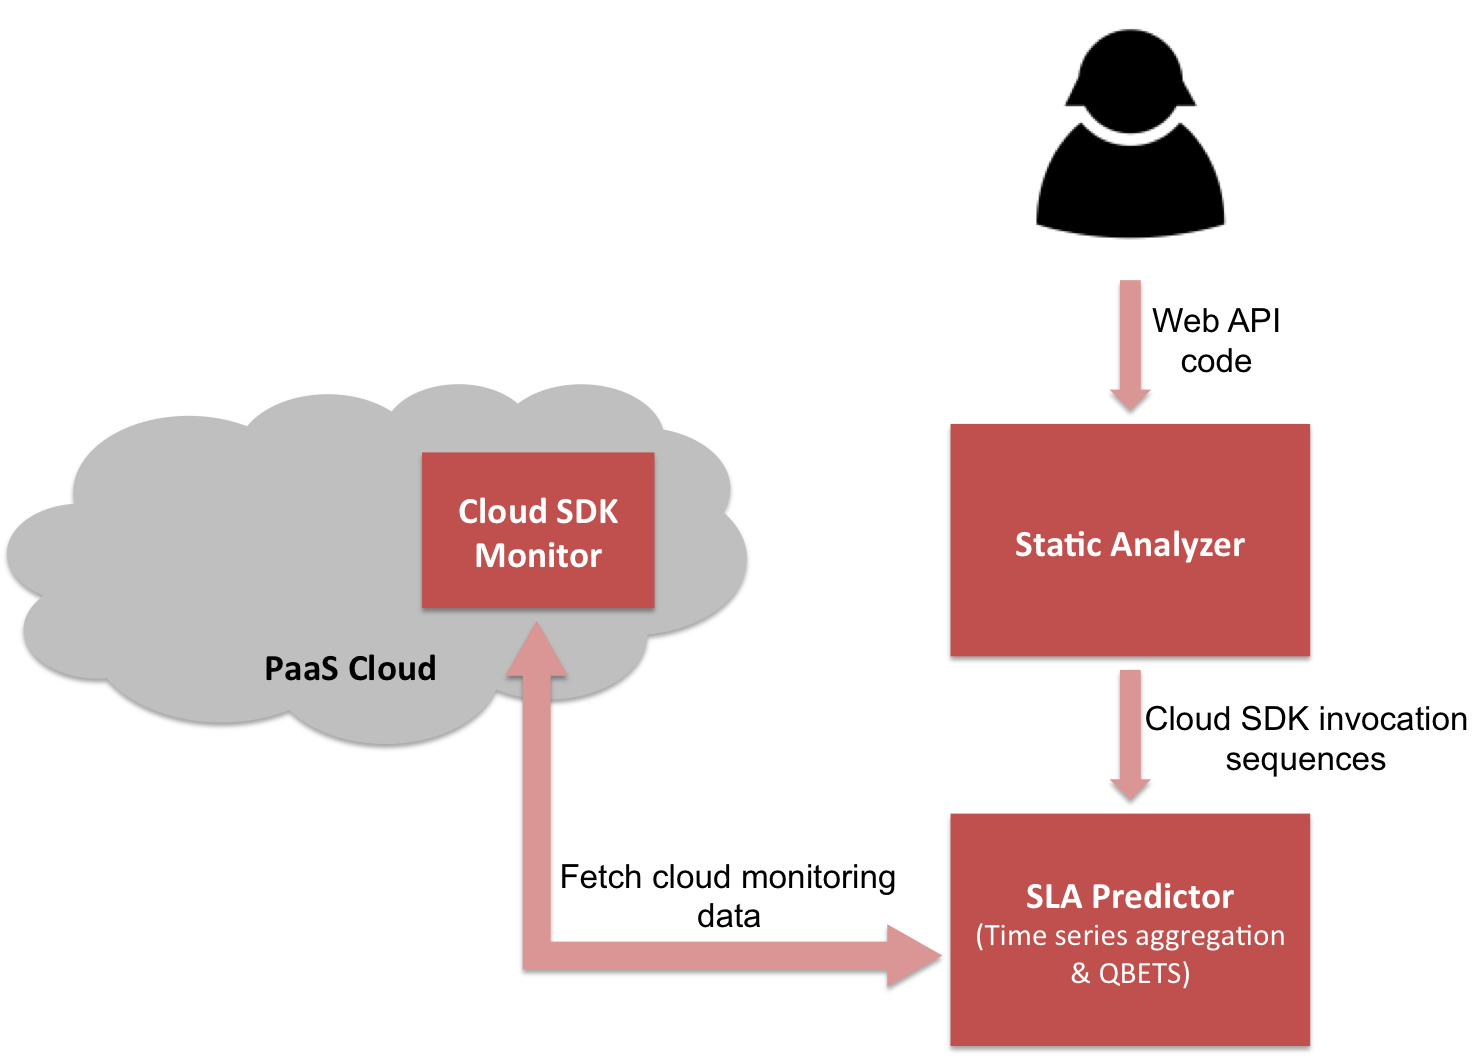
\includegraphics[scale=0.35]{apm_flow}
\caption{APM architecture and components interaction.}
\label{fig:apm_flow}
\end{figure}
Figure~\ref{fig:apm_flow} illustrates how the components interact with each other during the prediction making process.
The SLA prediction can be invoked when a web application is deployed to the PaaS cloud or at any time during the development process to give
developers insight into the worst-case response time of their applications.

When the prediction is invoked, it performs static analysis on all operations in the application. Next, it retrieves benchmarking data collected by
the monitoring agent for all PaaS service invocations. Finally, the QBETS analysis is applied to the data with the desired percentile and confidence value.
After the predictions are made, we can use the largest value across all application paths as the SLA prediction for a web application.

\subsection{Performance Anomaly Detection}
Numerous statistical models have been developed over time for detecting performance anomalies in running
applications. However, prior work has mostly focused on simple stand-alone applications. Few efforts have
extended this notion towards web applications, but web applications in PaaS clouds, for the most part,
is an uncharted territory. We intend to build on prior work regarding detecting performance anomalies in
web applications, and invent new mechanisms that can detect performance anomalies of PaaS-deployed
applications.

Such techniques must be able to detect a drop in performance level of an application, and then
determine if it occurred due to a change in the workload, or some system-level issue. This requires
correlating performance data of an application (e.g. response time), with workload information (e.g. number
of users). If a performance drop
occurred due to a system-level issue, we must further analyze the performance data concerning
PaaS kernel services. Note that the proposed APM collects such low-level information regarding
the PaaS kernel service invocations by applications. This information can be analyzed in relation 
to a detected performance anomaly to identify where the bottleneck is.

APM can also keep track of the sequences of PaaS kernel services invoked by a given application over time.
Each unique sequence represents the execution of a different path through the application code. 
This information is useful for
identifying the nature of the workload handled by a given application, and how it evolves with time. 
We can use novelty detection (a form of anomaly detection) to identify the execution of new, previously
unseen paths, which by themselves may be a sign of an anomaly.

\section{Conclusions}
As PaaS increased in popularity and use, the need 
for technologies to monitor and analyze the performance and behavior of
deployed applications has also grown. 
However, most PaaS clouds available today do not provide adequate support
for such analysis.
Therefore, we propose an application platform monitoring system that 
is able to take advantage of PaaS cloud features, but that is portable
across them.

To provide comprehensive full stack monitoring and analytics, 
the APM we propose provides four major functions:
data collecting, data storage, data processing, and data visualization. 
We describe the necessary organization of
these functions, and illustrate how these functions work as 
a component in the system. Also, by providing the
architecture of typical PaaS and proposed APM, we illustrate how these functions can be built as components that
make APM can be easily integrated with any PaaS.

After investigating popular application performance data collection and analysis tools, we choose ElasticSearch for data management.
ElasticSearch provides powerful, easy to use indexing features and scalability. We also choose to collect data via custom agents and Logstash.
Logstash supports a variety of standard log formants,
and is easy to customize the configuration to collect a variety of key data.

\bibliography{references}
\bibliographystyle{plain}

\end{document}
